\chapter{Comparaison entre Gadget et un code Vlasov\label{Chap::VlasovGadget}}
	\minitoc%

	% \todo[inline]{Ce chapitre en est à peine à son premier jet. Toutes les figures ne sont pas encore commenté (ça arrivera dans le courant de la
	% semaine). Il manque aussi les figures contenant tous les $j$ sommé.}

	% Une des questions qui se posent avec notre approche concerne sa validité. En effet, à quel point gadget peut il
	% être proche d'un programme résolvant directement les équations de Vlasov-Poisson. Dans ce chapitre, nous tentons
	% d'apporter des éléments de réponse.

	% Avant de présenter les résultats obtenus à propos de notre instabilité, nous allons présenter un travail que nous avons effectué en parallèle
	Dans ce chapitre, nous allons présenter un travail que nous avons effectué en parallèle
	avec Stéphane Colombi, Thierry Sousbie et Sébastien Peirani. Nous avons voulu comparer les résultats donnés par un code résolvant
	numériquement l'équation de Vlasov pour un système sphérique (écrit par Thierry Sousbie en se basant sur~\cite{1983PASJ...35..547F}) et le
	code $N$-corps \textsc{gadget-2}.

	Pour comparer nos simulations, nous regarderons la correspondance entre l'espace des phases $(r, v_r)$ pour $j=0,425$, l'espace
	des phases intégré sur $j$ et le profil de densité de l'objet. Nous effectuerons ces comparaison à différents temps afin
	de montrer que nous obtenons bien le même comportement au cours de l'évolution du système. La simulation \textsc{gadget-2} utilisée ici comporte $10^6$
	particules. L'article associé étudie aussi l'évolution de simulations composées de $10^5$ et $10^7$ particules.

	Tous les diagrammes de l'espace des phases que nous allons étudier présenterons à gauche la simulation Vlasov et à droite la simulation
	\textsc{gadget-2}, sauf si contre indication. Tous utilisent la même échelle de couleurs pour une même simulation. Le système d'unité utilisé
	est le même que~\citet{1983PASJ...35..547F}.

	\section{Description du code Vlasov}

		Nous considérons un système à symétrie sphérique. L'équation de Vlasov s'écrit:
		\begin{align}
			\pderivn{f}{t} + v_r\pderivn{f}{r} + \(\dfrac{j^2}{r^3} - \dfrac{GM(r)}{r^2}\)\pderivn{f}{v_r} = 0\label{Eq::ValGad::Pois}
		\end{align}
		avec $f = f(r, u, j, t)$ la fonction de distribution dans l'espace des phases du système au temps $t$, $r$ le rayon de l'objet, $v_r$
		la vitesse radiale et $j$ le moment angulaire. La fonction $M(r)$ donne la masse contenue à l'intérieur de la sphère de rayon $r$.

		Pour résoudre l'équation, l'espace des phases $\(r, v_r, j\)$ est discrétisé sur un maillage tridimensionnel tel que $(r, v_r,
		j)\in\(\left[r_\mathrm{min}; r_\mathrm{max}\right], \left[-v_r^\mathrm{max}; v_r^\mathrm{max}\right], \left[0;
		j_\mathrm{max}\right]\)$ avec $r$ évoluant logarithmiquement. Chaque point du maillage est considéré comme une particule.
		L'équation~\refeq{Eq::ValGad::Pois} est séparée en deux opérateurs:
		\begin{itemize}
			\item un premier opérateur permet d'obtenir la trajectoire d'une particule libre:
				\begin{align*}
					\pderivn{f}{t} + v_r\pderivn{f}{r} + \dfrac{j^2}{r^3}\pderivn{f}{u} = 0
				\end{align*}
			\item un second permettant de calculer l'accélération:
				\begin{align*}
					\pderivn{f}{t} - \dfrac{GM(r)}{r^2}\pderivn{f}{v_r} = 0
				\end{align*}
		\end{itemize}
		Ces deux opérateurs, alliés à un schéma de type \og\sm\fg, vont permettre de faire évoluer la position en chaque point du maillage du
		temps $t$ au temps $t+dt$. Puis, profitant du fait que toutes les couches de moment angulaire sont indépendantes des autres, une
		interpolation de la fonction de distribution dans le plan $\(r, v_r\)$ pour chaque $j$ permet de reconstruire le maillage.

		L'axe selon $r$ évoluant logarithmiquement, un problème va se poser lorsque $r\to0$. Pour l'éviter, nous faisons l'approximation que
		les particules à l'intérieur du rayon $r_\mathrm{min}$ sont libres. Ce rayon doit donc être suffisamment petit pour que cette approximation
		soit vérifiée, mais suffisamment grand pour éviter la divergence du logarithme.
		% toutes les particules passant sous ce rayon $r_\mathrm{min}$ puissent évoluer comme des particules libres.

		Plus de détails sur le fonctionnement du code pourront être trouvés dans l'article associé à cette étude (référence?). Pour effectuer
		la comparaison de ce code à \textsc{gadget-2}, nous allons utiliser une sphère de Hénon de viriel $\gamma$. À cause de certaines limitations
		inhérentes à l'interpolation, nous avons dû lisser cette sphère en multipliant la fonction de distribution par la fonction:
		\begin{align*}
			g(r) = \mathrm{erf}\( \dfrac{R - r }{ r_\epsilon }\) + 1
		\end{align*}
		avec $R$ est le rayon de l'objet et $r_\epsilon$ le rayon sur lequel la sphère sera lissée.

		Dans les sections suivantes, nous allons comparer ces deux codes en utilisant deux rapports du viriel: $\gamma=-0,5$ et $\gamma=-0,1$.
		% l'évolution de la sphère de Hénon avec un viriel de $\gamma=-0,5$ puis nous
		% enchaînerons sur une comparaison utilisant un viriel de $\gamma=-0.1$.

	\section{Tests préliminaire}
		Avant de comparer ces deux codes, nous allons vérifier deux points. Le premier est l'effet du lissage de la force $\epsilon$ sur
		l'évolution de la sphère de Hénon. Ensuite, nous vérifierons que les simulations \textsc{Gadget-2} conserve la sphéricité et
		l'isotropie de l'objet.

		\subsection{Effet du lissage de la force}

			Un paramètre important de la simulation va être le paramètre de lissage de la force $\epsilon$. Ce paramètre va influencer sur
			la dynamique en donnant ou retirant de l'importance au collision. Nous avons donc effectué des simulations d'une sphère de
			Hénon lissée, de viriel $\gamma=-0,5$, avec différents $\epsilon$. La figure~\ref{Fig::ValGad::0.5::SoftAll} montre l'espace
			des phases pour chaque valeur de $\epsilon$ testées.
			\begin{figure}[htbp]
				\begin{subfigure}{0.5\linewidth}
					\centering 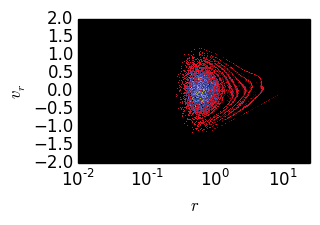
\includegraphics{{vlasov_gadget/Vlasov_0.5_Soft/CompVlasGad_512_0.5_0.0001}.png}
					\centering \caption{$\epsilon=10^{-4}$\label{Fig::ValGad::0.5::Soft1}}
				\end{subfigure}\hfill
				\begin{subfigure}{0.5\linewidth}
					\centering 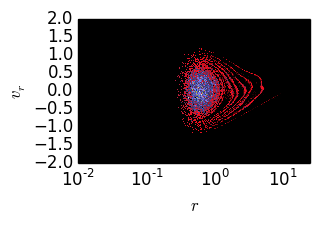
\includegraphics{{vlasov_gadget/Vlasov_0.5_Soft/CompVlasGad_512_0.5_0.001}.png}
					\centering \caption{$\epsilon=10^{-3}$\label{Fig::ValGad::0.5::Soft2}}
				\end{subfigure}
				\begin{subfigure}{0.5\linewidth}
					\centering 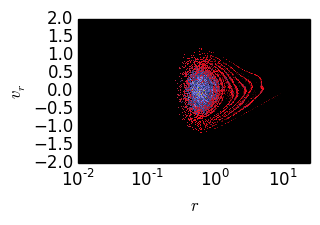
\includegraphics{{vlasov_gadget/Vlasov_0.5_Soft/CompVlasGad_512_0.5_0.01}.png}
					\centering \caption{$\epsilon=10^{-2}$\label{Fig::ValGad::0.5::Soft3}}
				\end{subfigure}\hfill
				\begin{subfigure}{0.5\linewidth}
					\centering 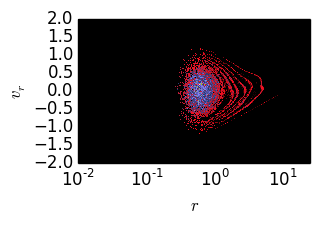
\includegraphics{{vlasov_gadget/Vlasov_0.5_Soft/CompVlasGad_512_0.5_0.1}.png}
					\centering \caption{$\epsilon=10^{-1}$\label{Fig::ValGad::0.5::Soft4}}
				\end{subfigure}
				\caption{Représentation de l'espace des phases à $j=0.425$ et $t=45$ pour $\gamma=-0,5$ et différents
					$\epsilon$.\label{Fig::ValGad::0.5::SoftAll}}
			\end{figure}
			Nous pouvons voir sur ces figures que l'espace des phases est très similaire, et ne semble pas dépendre de la valeur de
			$\epsilon$. Les enroulements présentent les mêmes variations et creux quelque soit la valeur de $\epsilon$.

			Dans la suite, nous prendrons $\epsilon=10^{-3}$. Cette valeur est légèrement différente de celle utilisée pour les simulations
			de l'article.

		\subsection{Sphéricité et isotropie}
			La symétrie sphérique est imposée par le code Vlasov.
			Nous allons donc vérifier que notre simulation conserve sa symétrie sphérique.
			Dans le même temps, nous allons vérifier que le résultat de l'effondrement de la sphère de Hénon reste isotrope.

			C'est ce que montrent les figures~\ref{Fig::VlaGad::SpheTest::AR} et~\ref{Fig::VlaGad::SpheTest::Aniso} pour $\gamma=-0,5$.
			\begin{figure}[htbp]
				\begin{minipage}{0.44\linewidth}
					\begin{center}
					\centering 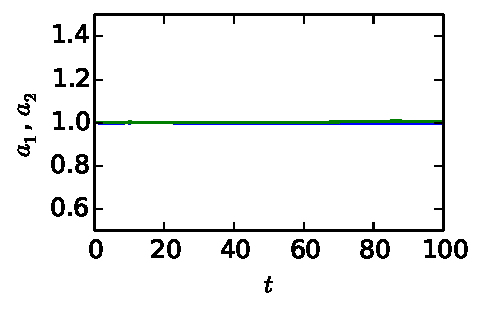
\includegraphics{{vlasov_gadget/AxialRatio_0.5}.pdf}
					\centering \caption{Évolution des rapports d'axes $a_1$ et $a_2$ pour $\gamma=-0,5$.\label{Fig::VlaGad::SpheTest::AR}}
					\end{center}
				\end{minipage}\hfill
				\begin{minipage}{0.45\linewidth}
					\begin{center}
					\centering 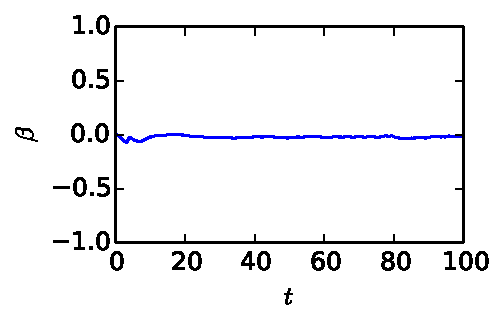
\includegraphics{{vlasov_gadget/Anisotropy_0.5}.pdf}
					\centering \caption{Évolution de l'anisotropie pour $\gamma=-0,5$.\label{Fig::VlaGad::SpheTest::Aniso}}
					\end{center}
				\end{minipage}
			\end{figure}
			La première montre l'évolution des rapports d'axes au cours du temps. Ils restent tous deux très proches de $1$. La sphère de Hénon
			reste bien sphérique tout du long de son évolution. La figure~\ref{Fig::VlaGad::SpheTest::Aniso} montre l'évolution de
			l'anisotropie au cours du temps. Son évolution confirme que la sphère reste isotrope.

			Les figures~\ref{Fig::VlaGad::SpheTest::AR0.1} et~\ref{Fig::VlaGad::SpheTest::Aniso0.1} montrent, respectivement, le comportement
			des rapports d'axes et de l'anisotropie pour la simulation de viriel $\gamma=-0,1$.
			\begin{figure}[htbp]
				\begin{minipage}{0.44\linewidth}
					\begin{center}
					\centering 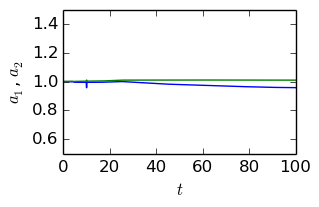
\includegraphics{{vlasov_gadget/AxialRatio_0.1}.pdf}
					\centering \caption{Évolution des rapports d'axes $a_1$ et $a_2$ pour
					$\gamma=-0,1$.\label{Fig::VlaGad::SpheTest::AR0.1}}
					\end{center}
				\end{minipage}\hfill
				\begin{minipage}{0.45\linewidth}
					\begin{center}
					\centering 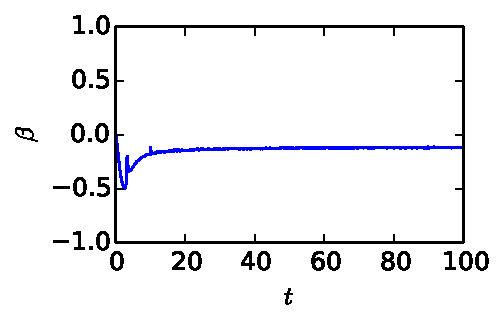
\includegraphics{{vlasov_gadget/Anisotropy_0.1}.pdf}
					\centering \caption{Évolution de l'anisotropie pour $\gamma=-0,1$.\label{Fig::VlaGad::SpheTest::Aniso0.1}}
					\end{center}
				\end{minipage}
			\end{figure}
			Les rapports d'axes nous apprennent qu'une légère déformation de l'objet (inférieur à $3\%$) apparaît. Cette
			déformation est suffisamment faible pour que l'on puisse considérer l'objet comme sphérique. L'anisotropie, par contre, se
			stabilise à $-0,1$ après l'effondrement au lieu de $0$. Notre sphère de Hénon présente une légère anisotropie radiale dans
			l'espace des vitesses.
			% L'évolution de ces trois observables confirment bien que l'objet reste sphérique et isotrope pour cette valeur de $\gamma$.


	\section{Comparaison entre les simulations Vlasov et \textsc{Gadget-2}}
		\subsection{Pour $\gamma = -0,5$}

		Les figures~\ref{Fig::ValGad::0.5::t0}, \ref{Fig::ValGad::0.5::t13} et~\ref{Fig::ValGad::0.5::t45} montre l'évolution de l'espace des
		phases pour $j=0,425$ au cours de l'évolution. À l'exception d'un effet de diffusion apparaissant dans le code Vlasov, l'accord entre
		les deux simulations est très bon jusqu'à $t=45$. À ce moment, les effets de diffusion sont clairement visibles sur les enroulements
		extérieurs. D'autres différences apparaissent: certains creux de la simulation \textsc{Gadget-2} semblent en avance par rapport à
		Valsov. De la même façon, certaines des bosses sur les enroulements extérieurs sont décalées vers de plus grandes vitesses radiales,
		et de plus faibles vitesses radiales pour les enroulements les plus intérieurs. 

		Les figures~\ref{Fig::ValGad::0.5::Density::t0}, \ref{Fig::ValGad::0.5::Density::t13} et~\ref{Fig::ValGad::0.5::Density::t45} nous
		informent sur l'évolution du profil de densité. Exceptés au centre et sur le bord du système, où le nombre de particules devient trop
		faible, la variation relative entre les deux simulations est au pire de l'ordre de $25\%$.

		Le dernier jeu de figures (\ref{Fig::VlaGad::0.5::JAll::t0}, \ref{Fig::VlaGad::0.5::JAll::t13} et~\ref{Fig::VlaGad::0.5::JAll::t45})
		concerne l'espace des phases intégré. Ces trois figures confirment ce que nous avons dit précédemment, l'accord entre les deux
		simulations est excellent, jusqu'à $t=45$ où le décalage entre les deux simulations apparaît nettement.
			
		L'évolution des deux simulations semble commencer à diverger pour $t=45$. Ce décalage n'apparait pas dans les simulations présentées
		dans notre article. Les principales différences entre ces simulations et celles de l'article sont $\epsilon$ et le pas de temps
		maximal autorisé. Nous avons déjà montré que $\epsilon$ n'avait pas d'influence importante sur la dynamique. La dernière possibilité
		est donc le pas de temps, dix fois supérieur aux simulations montrées dans l'article.

		\begin{figure}[htbp]
			\begin{minipage}{1.00\linewidth}
				\centering \includegraphics[width=\linewidth]{{CompVlasGad_t_0_512_0.5}.png}
				\caption{Comparaison de l'espace des phases entre le code Vlasov (à gauche) et le code Gadget (à droite), à
				$t=0$ et pour $j=0,425$.\label{Fig::ValGad::0.5::t0}}
			\end{minipage}\hfill
			\begin{minipage}{1.00\linewidth}
				\centering \includegraphics{{CompVlasGad_Density_0.5_t_0_error}.pdf}
				\caption{Comparaison du profil de densité entre le code Vlasov (en bleu) et le code gadget (en vert), pour
				$t=0$.\label{Fig::ValGad::0.5::Density::t0}}
			\end{minipage}
		\end{figure}
		\begin{figure}[htbp]
			\begin{minipage}{1.00\linewidth}
				\centering \includegraphics[width=\linewidth]{{CompVlasGad_t_13_512_0.5}.png}
				\caption{Comparaison de l'espace des phases entre le code Vlasov (à gauche) et le code Gadget (à droite), à $t=13$ et
				pour $j=0,425$.\label{Fig::ValGad::0.5::t13}}
			\end{minipage}\hfill
			\begin{minipage}{1.00\linewidth}
				\centering \includegraphics{{CompVlasGad_Density_0.5_t_13_error}.pdf}
				\caption{Comparaison du profil de densité entre le code Vlasov (en bleu) et le code gadget (en vert), pour
				$t=13$.\label{Fig::ValGad::0.5::Density::t13}}
			\end{minipage}
		\end{figure}
		\begin{figure}[htbp]
			\begin{minipage}{1.00\linewidth}
				\centering \includegraphics[width=\linewidth]{{CompVlasGad_t_45_512_0.5}.png}
				\caption{Comparaison de l'espace des phases entre le code Vlasov (à gauche) et le code Gadget (à droite), à $t=45$ et
				pour $j=0,425$.\label{Fig::ValGad::0.5::t45}}
			\end{minipage}\hfill
			\begin{minipage}{1.00\linewidth}
				\centering \includegraphics{{CompVlasGad_Density_0.5_t_45_error}.pdf}
				\caption{Comparaison du profil de densité entre le code Vlasov (en bleu) et le code gadget (en vert), pour
				$t=45$.\label{Fig::ValGad::0.5::Density::t45}}
			\end{minipage}
		\end{figure}

		\begin{figure}[htbp]
			\begin{subfigure}{1.0\linewidth}
				\centering \includegraphics[scale=0.75]{{CompVlasGad_t_0_512_0.5_Jall-v2}.png}
				\caption{$t=0$.\label{Fig::VlaGad::0.5::JAll::t0}}
			\end{subfigure}
			\begin{subfigure}{1.0\linewidth}
				\centering \includegraphics[scale=0.75]{{CompVlasGad_t_13_512_0.5_Jall-v2}.png}
				\caption{$t=13$.\label{Fig::VlaGad::0.5::JAll::t13}}
			\end{subfigure}
			\begin{subfigure}{1.0\linewidth}
				\centering \includegraphics[scale=0.75]{{CompVlasGad_t_45_512_0.5_Jall-v2}.png}
				\caption{$t=45$.\label{Fig::VlaGad::0.5::JAll::t45}}
			\end{subfigure}
			\caption{Espace des phases intégré sur $j$ pour $\gamma=-0,5$. La simulation Vlasov se trouve à gauche, à droite la simulation gadget.}
		\end{figure}

		\subsection{Pour $\gamma = -0,1$}

		Les résultats associés à ce viriel sont similaires mais un peu plus complexes. En effet, si nous regardons le profil de densité à
		différents temps (voir les figures~\ref{Fig::ValGad::0.1::Density::t0}, \ref{Fig::ValGad::0.1::Density::t5}
		et~\ref{Fig::ValGad::0.1::Density::t25}), l'accord est excellent (toujours à l'exception du centre et du bord du système). Lorsque
		l'on s'intéresse à l'espace des phases, les temps $t=0$ (figure~\ref{Fig::ValGad::0.1::t0} et~\ref{Fig::VlaGad::0.1::JAll::t0}) et
		$t=5$ (figure~\ref{Fig::ValGad::0.1::t5} et~\ref{Fig::VlaGad::0.1::JAll::t5}) montrent là encore un excellent accord. Au temps $t=25$
		(figure~\ref{Fig::ValGad::0.1::t25} et~\ref{Fig::VlaGad::0.1::JAll::t25}), les espaces des phases semblent en bon accord, mais la
		simulation Vlasov montre un effet d'aliasing numérique. Dans le même temps, la simulation \textsc{Gadget-2} développe une instabilité
		(visible sur les enroulements extérieurs) qui n'est pas présente dans la simulation Vlasov.

		Les détails à propos du développement de l'instabilité des simulations \textsc{Gadget-2} pourront être trouvés dans l'appendice A de
		l'article (référence encore et toujours). Cette instabilité est due à la nature particulaire de la simulation. L'instabilité
		apparaissant dans la simulation Vlasov vient d'un mauvais échantillonnage du moment angulaire.

		\begin{figure}[htbp]
			\begin{minipage}{1.00\linewidth}
				\centering \includegraphics[width=\linewidth]{{CompVlasGad_t_0_512_0.1}.png}
				\caption{Comparaison de l'espace des phases entre le code Vlasov (à gauche) et le code Gadget (à droite), à $t=0$ et pour $j=0,425$.\label{Fig::ValGad::0.1::t0}}
			\end{minipage}\hfill
			\begin{minipage}{1.00\linewidth}
				\centering \includegraphics{{CompVlasGad_Density_0.1_t_0_error}.pdf}
				\caption{Comparaison du profil de densité entre le code Vlasov (en bleu) et le code gadget (en vert), pour $t=0$.\label{Fig::ValGad::0.1::Density::t0}}
			\end{minipage}
		\end{figure}
		\begin{figure}[htbp]
			\begin{minipage}{1.00\linewidth}
				\centering \includegraphics[width=\linewidth]{{CompVlasGad_t_5_512_0.1}.png}
				\caption{Comparaison de l'espace des phases entre le code Vlasov (à gauche) et le code Gadget (à droite), à $t=5$ et pour $j=0,425$.\label{Fig::ValGad::0.1::t5}}
			\end{minipage}\hfill
			\begin{minipage}{1.00\linewidth}
				\centering \includegraphics{{CompVlasGad_Density_0.1_t_5_error}.pdf}
				\caption{Comparaison du profil de densité entre le code Vlasov (en bleu) et le code gadget (en vert), pour $t=5$.\label{Fig::ValGad::0.1::Density::t5}}
			\end{minipage}
		\end{figure}
		\begin{figure}[htbp]
			\begin{minipage}{1.00\linewidth}
				\centering \includegraphics[width=\linewidth]{{CompVlasGad_t_25_512_0.1}.png}
				\caption{Comparaison de l'espace des phases entre le code Vlasov (à gauche) et le code Gadget (à droite), à $t=25$ et pour $j=0,425$.\label{Fig::ValGad::0.1::t25}}
			\end{minipage}\hfill
			\begin{minipage}{1.00\linewidth}
				\centering \includegraphics{{CompVlasGad_Density_0.1_t_25_error}.pdf}
				\caption{Comparaison du profil de densité entre le code Vlasov (en bleu) et le code gadget (en vert), pour $t=25$.\label{Fig::ValGad::0.1::Density::t25}}
			\end{minipage}
		\end{figure}
		% \begin{figure}[htbp]
			% \begin{minipage}{1.00\linewidth}
				% \centering \includegraphics[width=\linewidth]{{CompVlasGad_t_35_512_0.1}.png}
				% \caption{Comparaison de l'espace des phases entre le code vlasov (à gauche) et le code Gadget (à droite), à $t=35$ et
				% pour $j=0,425$.\label{Fig::ValGad::0.1::t35}}
			% \end{minipage}\hfill
			% \begin{minipage}{1.00\linewidth}
				% \centering \includegraphics{{CompVlasGad_Density_0.1_t_35_error}.pdf}
				% \caption{Comparaison du profil de densité entre le code vlasov (en bleu) et le code gadget (en vert), pour $t=35$.\label{Fig::ValGad::0.1::Density::t35}}
			% \end{minipage}
		% \end{figure}

		\begin{figure}[htbp]
			\begin{subfigure}{1.0\linewidth}
				\centering \includegraphics[scale=0.75]{{CompVlasGad_t_0_512_0.1_Jall-v2}.png}
				\caption{$t=0$.\label{Fig::VlaGad::0.1::JAll::t0}}
			\end{subfigure}
			\begin{subfigure}{1.0\linewidth}
				\centering \includegraphics[scale=0.75]{{CompVlasGad_t_5_512_0.1_Jall-v2}.png}
				\caption{$t=5$.\label{Fig::VlaGad::0.1::JAll::t5}}
			\end{subfigure}
			\begin{subfigure}{1.0\linewidth}
				\centering \includegraphics[scale=0.75]{{CompVlasGad_t_25_512_0.1_Jall-v2}.png}
				\caption{$t=25$.\label{Fig::VlaGad::0.1::JAll::t25}}
			\end{subfigure}
			\caption{Espace des phases intégré sur $j$ pour $\gamma=-0,1$. La simulation Vlasov se trouve à gauche, à droite la simulation gadget.}
		\end{figure}



	Au cours des deux dernières sous-sections, nous venons de comparer deux simulations, l'une effectuée avec un code Vlasov, l'autre avec
	\textsc{Gadget-2}. L'accord entre ces deux simulations, même à faible viriel, est excellent. Pour le cas $\gamma=-0.1$, il est difficile de
	réellement conclure, puisque des instabilités numériques se produisent relativement tôt dans la simulation, même si la correspondance observée
	avant semble optimiste.












		% Le premier temps que nous regardons est $t=0$. La figure~\ref{Fig::ValGad::0.5::t0} Du côté du profil de densité
		% (figure~\ref{Fig::ValGad::0.5::Density::t0}), l'accord est très bon, excepté au centre du système où le manque de particules empêche
		% le calcul précis de la densité.
		% Le deuxième temps que nous avons choisi de montrer se situe peu après la fin de l'effondrement de la sphère de Hénon. Le nombre
		% d'enroulement présent sur les graphiques de la figure~\ref{Fig::ValGad::0.5::t13} sont les mêmes. Par contre, l'enroulement central
		% donne de la simulation gadget semble un peu en avance sur la simulation vlasov. Ce qui semble confirmé par le \og{}bras\fg s'étendant
		% jusqu'à $r=3$ pour la simulation vlasov et jusqu'à $r=4$ pour la simulation gadget.
		% Les profils de densité présenté sur la figure~\ref{Fig::ValGad::0.5::Density::t13} montre par contre un très bon accord, excepté au
		% bord du système, où le nombre de particules recommence alors à faiblir. L'extension du système en $r$ est aussi visible.
		% Cette extension du profil peut-être expliqué par l'éjection d'une fraction des particules hors du système suite aux collisions se
		% produisant dans le système.
		% Pour terminer la comparaison à ce viriel, nous regardons ce qu'il se passe à $t=45$. À ce moment, le système a eu le temps de se
		% stabiliser. Nous remarquons, en regardant la figure~\ref{Fig::ValGad::0.5::t45}, que la simulation gadget présente des
		% \og{}vaguelettes\fg sur les enroulements extérieurs qui semble en avance sur la simulation vlasov.


		% Le premier temps que nous regardons est $t=0$. La figure~\ref{Fig::ValGad::0.1::t0} montre l'espace des phases pour les conditions
		% initiales. La première chose à noter concerne la différence apparente concernant le maximum de la fonction de distributions. Cette
		% différence est dû au faible nombre de particules présentes dans la couche de $j$ choisi. Excepté ce point, nous retrouvons bien la
		% croissance progressive du nombre de particule ainsi qu'un étalement progressif des vitesses radiales quand $r$ augmente.
		% Du côté du profil de densité (figure~\ref{Fig::ValGad::0.1::Density::t0}), l'accord est très bon, excepté au centre du système où le manque de particules empêche le calcul précis
		% de la densité.

		% Le deuxième temps que nous avons choisi de montrer se situe peu après la fin de l'effondrement de la sphère de Hénon. Le nombre
		% d'enroulement présent sur les graphiques de la figure~\ref{Fig::ValGad::0.1::t13} sont les mêmes. Par contre, l'enroulement central
		% donne de la simulation gadget semble un peu en avance sur la simulation vlasov. Ce qui semble confirmé par le \og{}bras\fg s'étendant
		% jusqu'à $r=3$ pour la simulation vlasov et jusqu'à $r=4$ pour la simulation gadget.
		% Les profils de densité présenté sur la figure~\ref{Fig::ValGad::0.1::Density::t13} montre par contre un très bon accord, excepté au
		% bord du système, où le nombre de particules recommence alors à faiblir. L'extension du système en $r$ est aussi visible.
		% Cette extension du profil peut-être expliqué par l'éjection d'une fraction des particules hors du système suite aux collisions se
		% produisant dans le système.

		% Pour terminer la comparaison à ce viriel, nous regardons ce qu'il se passe à $t=45$. À ce moment, le système a eu le temps de se
		% stabiliser. Nous remarquons, en regardant la figure~\ref{Fig::ValGad::0.1::t45}, que la simulation gadget présente des
		% \og{}vaguelettes\fg sur les enroulements extérieurs qui semble en avance sur la simulation vlasov.
